\documentclass[fleqn,reqno,10pt,draft]{article}

\usepackage{myarticlestyledefault}


\usepackage{mypackages}
\usepackage{mycommands}
\usepackage{myenvironments}

\usepackage[]{svninfo}
\usepackage{subfig}



\newcommand{\lit}{\acro{lit}}
\newcommand{\glb}{\acro{glb}}
\newcommand{\loc}{\acro{loc}}

\newcommand{\as}{\acro{as}}
\renewcommand{\es}{\acro{es}}
\renewcommand{\AE}{\as}
\newcommand{\GE}{\es}

\newcommand{\lc}{\acro{lc}}
\newcommand{\ec}{\acro{ec}}
\newcommand{\LC}{\lc}
\newcommand{\EC}{\ec}


\DefineNamedColor{named}{mycol}{cmyk}{0.6,0.6,0,0}
\DefineNamedColor{named}{mygray}{cmyk}{0.05,0.05,0.05,0.05}
\DefineNamedColor{named}{mygraylight}{cmyk}{0.017,0.017,0.017,0.017}

\newcommand{\mymark}[1]{{\color{mycol}{#1}}}
\newcommand{\exh}{\ensuremath{\mathrm{Exh}}}
\newcommand{\alt}{\ensuremath{\mathrm{Alt}}}


\title{Scalar Items in Embedded Position: {A}nother Experimental Approach}
\author{Fabian Schlotterbeck, Michael Franke and Petra Augurzky}
\date{}

\begin{document}
\maketitle


\begin{abstract}
  \dots make concrete \dots
\end{abstract}

\svnInfo $Id$

\section{Introduction}
\label{sec:introduction}

This paper deals with the interpretation of two types of
sentences, namely:

\begin{exe}
\ex \label{bsp:AE}
  \mymark{All} of the students read \mymark{some} of the
  papers. \hfill (\AE)
\ex \label{bsp:GE} 
  \mymark{Exactly one} of the students read \mymark{some} of the
  papers. \hfill (\GE)
\end{exe}

\noindent In \as-sentences the scalar item \emph{some} like takes
scope under universal quantifier \emph{all}. In \es-sentences
\emph{some} takes scope under non-monotonic quantifier \emph{exactly
  one}. These sentences are interesting, because, according to current
pragmatic theorizing, they may have at least three conceivable
readings. The main question we are interested in here is which of
these three conceivable readings is available to subjects na\"{i}ve to
all pragmatic theory. We are moreover interested in the more refined
question which of the available readings na\"{i}ve subjects prefer.

What are the possible readings of \as- and \es-sentences? Scalar
\emph{some} is usually assumed to receive a semantic interpretation
similar to logical $\exists$, so that the sentence \emph{Some boys
  cried} is literally true in a situation where all boys cried. But it
is also known to invite upper-bounding inferences in plain utterances:

\begin{exe}
  \ex \label{bsp:Plain-SI}
    \begin{xlist}
      \ex \label{bsp:Plain-SI-Target} Hans solved some of the problems.
      \ex \label{bsp:Plain-SI-Implicature} $\implicates$ Hans solved some but not all of the problems.
    \end{xlist}
\end{exe}

\noindent The classical explanation of this inference, following the
pioneering work of \citet{Grice1975:Logic-and-Conve}, has it that
(\ref{bsp:Plain-SI-Implicature}) is a pragmatic inference, a so-called
\emph{quantity implicature}, derived by an abductive inference as the
best explanation of why am informed, knowledgable and cooperative
speaker has uttered (\ref{bsp:Plain-SI-Target}) when she could also
have uttered the semantically stronger and relevant:\dn{redo labels of
  examples}

\begin{exer}{bsp:Plain-SI}
  \ex
    \begin{xlist}
      %% DiRTY !!
      \addtocounter{xnumii}{2}
      \ex \label{bsp:Plain-SI-Alternative} Hans solved all of the problems.
    \end{xlist}
\end{exer}

\noindent If this upper-bounding inference would occur often and
systematically enough, then it may well be that also embedded
occurrences of \emph{some} get enriched, in some fashion or other, to
contribute the enriched meaning \emph{some but not all} also under the
scope of other logical operators. Indeed, even
\citeauthor{Grice1975:Logic-and-Conve} envisaged this possibility when
he wrote: ``It may not be impossible for what starts life, so to
speak, as a conversational implicature to become conventionalized''
\citep[p.58]{Grice1975:Logic-and-Conve}. But then there are at least
three relevant candidate readings for \as- and \es-sentences: (i) a
\emph{literal reading} like in (\ref{bsp:AE-Literal}) and
(\ref{bsp:GE-Literal}) where \emph{some} has only its literal meaning;
(ii) a \emph{global reading} like in (\ref{bsp:AE-Global}) and
(\ref{bsp:GE-Global}) where, according to the Gricean intuition, we
enrich utterances of (\ref{bsp:AE}) and (\ref{bsp:GE}) with the
negation of alternativ utterances of the corresponding sentences
(\ref{bsp:AE-Alternative}) and (\ref{bsp:GE-Alternative}) where
\emph{some} is replaced by \emph{all}; and also (iii) a \emph{local
  reading} like in (\ref{bsp:AE-Local}) and (\ref{bsp:GE-Local}) where
\emph{some} is read to mean \emph{some but not all} in the scope of
the embedding quantifier.


\begin{exer}{bsp:AE}
  \ex \mymark{All} of the students read {\mymark{some}} of the
  papers. 

  \begin{xlist}
  \ex \label{bsp:AE-Literal} \mymark{All} of the students read
    {\mymark{some and maybe all}} of the papers. \hfill (\as-\lit)
  \ex \label{bsp:AE-Global}
    \mymark{All} of the students read \mymark{some and maybe all} 
    and  \hfill (\as-\glb)\\
    it's not the case that \mymark{all} of the students read \mymark{all} of the papers.
  \ex \label{bsp:AE-Local}
    \mymark{All} of the students read {\mymark{some  but not all}} of the
    papers. \hfill (\as-\loc)
  \end{xlist}
\end{exer}

\begin{exer}{bsp:GE}
\ex \mymark{Exactly one} of the students read {\mymark{some}} of the
  papers.

  \begin{xlist}
  \ex \label{bsp:GE-Literal} \mymark{Exactly one} of the students read
    {\mymark{some and maybe all}} of the papers. \hfill (\es-\lit)
  \ex \label{bsp:GE-Global}
    \mymark{Exactly one} of the students read \mymark{some and maybe all} 
    and  \hfill (\es-\glb)\\
    it's not the case that \mymark{exactly one} of the students read \mymark{all} of the papers.
  \ex \label{bsp:GE-Local}
    \mymark{Exactly one} of the students read {\mymark{some  but not all}} of the
    papers. \hfill (\es-\loc)
  \end{xlist}
\end{exer}


\begin{exe}
\ex \label{bsp:AE-Alternative} \mymark{All} of the students read
  {\mymark{all}} of the papers. 

\ex \label{bsp:GE-Alternative} \mymark{Exactly one} of the students
  read {\mymark{all}} of the papers.
\end{exe}

\noindent Section~\ref{sec:get-know-your} will discuss these reading
in more detail and, by giving some helpful illustrations, make clear
that these readings are all distinct but logically dependent
on each other in interesting ways.

The empirical questions we would like to ask, namely (i) which of
these readings are available, and (ii) which of the available ones are
the preferred interpretations, are highly relevant because they lie at
the heart of the current debate about the exact location and nature of
the interface between semantics and pragmatics. There are three major
camps which are ---more or less fiercely--- involved in this border
war, all of which make different predictions about availability and
preferences of readings. We will give a more detailed description of
the various theoretical positions below in
Section~\ref{sec:theories-predictions}, but on a first rough
approximation the situation is the following. 

Firstly, there are \mymark{pragmatic traditionalists} who seek to
conserve the spirit of \citeauthor{Grice1975:Logic-and-Conve}'s
(\citeyear{Grice1975:Logic-and-Conve}) original ideas as much as
possible
\citep[e.g.][]{Spector2006:Scalar-Implicat,Sauerland2004:Scalar-Implicat,Russell2006:Against-Grammat,vanRooijSchulz:ExhaustiveInterpretation,Geurts2010:Quantity-Implic,Franke2011:Quantity-Implic}. Traditionalists
happily acknowledge the existence of global readings, but might
consider local readings either unavailable or a beast distinct from
scalar implicatures. An often phrased intuition of the traditionalists
is that local readings, since they are special kinds of inferences,
require special intonation, in particular emphatic stress on the
scalar item.\dn{give references}

Opposed to that is the camp of \mymark{lexical conventionalists}
\citep[e.g.][]{LevinsonPresumptiveMeanings2000,Chierchia:2004_ScalarImplicatures}
who maintain that scalar \emph{some} is lexically ambiguous between
the standard logical meaning \emph{some and maybe all} and the
upper-bounded meaning \emph{some but not all}. As the latter is
considered a default, lexical conventionalism has no problem
accounting for local readings, and in fact would consider these the
preferred readings. 

Thirdly and finally, there is the camp of \mymark{grammaticalists} who
defend that the distribution of upper-bounded readings of \emph{some}
is best explained by postulating a silent operator, akin to the
meaning of the particle \emph{only}
\citep{Chierchia2006:Broaden-Your-Vi,Fox2007:Free-Choice-and,Magri2011:Another-Argumen,Sauerland2012:The-Computation,ChierchiaFox2008:The-Grammatical,Chierchia2012:FC-Nominals-and}. According
to the grammatical view, this silent operator may be applied in
compositional semantics also in the scope of other logical operators,
but, so as not to overgenerate readings, the availability of readings
is constraint by the \emph{strongest meaning hypothesis}
\citep{DalrympleKanazawa1998:Reciprocal-Expr}. Grammaticalist theories
predict that all three types of readings are available. Moreover,
according to the grammatical view, the local reading is preferred for
\as-sentences, while the global one is preferred for
\es-sentences. (More precisely, as we will see
Section~\ref{sec:theories-predictions}, depending on the variant of
the strongest meaning hypothesis employed, either the global reading
is predicted to be preferred for \es-sentences, or the global and the
local reading are predicted to be equally preferred.)

Due to its theoretical significance, a number of previous studies have
already probed into the availability of readings for \as- and
\es-sentences
\citep[e.g.][]{GeurtsPouscoulous2009:Embedded-Implic,CliftonDube2010:Embedded-Implic,ChemlaSpector2010:Experimental-Ev}. However,
as we will argue in Section~\ref{sec:previous-studies}, results have
not been as clear-cut as one might have hoped for. Even worse so,
taken in conjunction, the empirical evidence is inconclusive as to
whether local readings exist. We hypothesized that previous studies
might be insufficiently informative because of the focus on (variants
of) a picture-verification paradigm.\dn{relate to Bob van Tiel's
  work}  The problem is that in order to test the availability of
different candidate meanings different pictures have to be presented,
so that effects of pictorial complexity or stereotypicality could
never be ruled out entirely. Moreover, previous studies have only
accumulated limited evidence pertaining to the second question that
may help decide between theoretical positions, namely which of the
attested readings subjects prefer.

In reaction to this situation, we therefore studied a different mode
of visual presentation: subjects were presented with pictures that
were partly covered and could incrementally be uncovered at the
subjects' request; for each ((partially) covered) picture, subjects
had to decide whether they could already give a truth-value judgement
or needed more information.\dn{mention who else does this} This way we
obtained behavioral data that is both indicative of the reading
subjects assumed and independent of the complexity of the visual
stimulus. At the same time, we hypothesized that the incremental
nature of this task would shed light on the preferences over readings,
because the temporal distribution of truth-value judgments would give
away which reading subjects were waiting to evaluate, so to speak. To
test whether our method is indeed suitable to detect interpretation
preferences, we included ambiguous test items like
(\ref{bsp:target-related-filler}) which are known to preferentially
receive the late-closure reading in
(\ref{bsp:target-related-filler-LC}) and not the dispreferred, but
attested early-closure reading
(\ref{bsp:target-related-filler-EC}).\dn{insert references to
  literature on EC-LC processing}

\begin{exe}
\ex \label{bsp:target-related-filler} The letter is connected with circles and squares with
  suns.
  \begin{xlist}
  \ex \label{bsp:target-related-filler-LC} The letter is connected
    with squares with suns and circles. \hfill (\LC)
  \ex \label{bsp:target-related-filler-EC} The letter is connected
    with circles with suns and squares with suns. \hfill (\EC)
  \end{xlist}
\end{exe}

\noindent Finally, since it is often argued (see
Section~\ref{sec:theories-predictions}) that intonational stress on an
embedded scalar item can favor a local reading we presented sentence
auditorily and manipulated stress accordingly. The design of our
studies is detailed in Section XYZ.

\begin{itemize}
\item summarize results
\end{itemize}

The paper is structured as follows. Section~\ref{sec:get-know-your}
elaborates on the three kinds of relevant readings for our target
sentences. Section~\ref{sec:theories-predictions} works out the
different theoretical positions and their predictions about
availability and preference. Section~\ref{sec:previous-studies} recaps
the results of previous studies on this subject, arguing for the need
of a more refined methodology. Section~\ref{sec:design} describes our
experimental design. Section~\ref{sec:results} states our results,
which we discuss in Section~\ref{sec:discussion}.\dn{rephrase
  eventually}

\section{Get to know your readings}
\label{sec:get-know-your}

Three readings are \emph{prima facie} conceivable for the \as- and
\es-sentences in (\ref{bsp:AE}) and (\ref{bsp:GE}). These are
logically distinct, but also logically dependent in intricate ways. To
see this, let us look at each kind of sentence in turn.

\subsection{\as-sentences}
\label{sec:as-sentences}

An \as-sentence like (\ref{bsp:AE}) has a literal reading as in
(\ref{bsp:AE-Literal}), a global reading as in (\ref{bsp:AE-Global})
and a local reading as in (\ref{bsp:AE-Local}).

\begin{exer}{bsp:AE}

  \ex \mymark{All} of the students read {\mymark{some}} of the
  papers. 

  \begin{xlist}
  \ex \mymark{All} of the students read
    {\mymark{some and maybe all}} of the papers. \hfill (\as-\lit)
  \ex
    \mymark{All} of the students read \mymark{some and maybe all} 
    and  \hfill (\as-\glb)\\
    it's not the case that \mymark{all} of the students read \mymark{all} of the papers.
  \ex
    \mymark{All} of the students read {\mymark{some  but not all}} of the
    papers. \hfill (\as-\loc)
  \end{xlist}
\end{exer}

\noindent These readings stand in a strict entailment relation,
namely the local reading asymmetrically entails the global reading,
which asymmetrically entails the literal reading:
\begin{exe}
  \ex \label{bsp:Entailments-AS} \loc $\subset$ \glb $\subset$ \lit
\end{exe}
That \glb $\subseteq$ \lit is obvious, given that \glb is defined as the
conjunction of \lit and the negated (relevant/feasible) alternative(s)
of the to-be-interpreted utterance. The entailment is asymmetric,
because the information that not all of the students read all of the
papers is not entailed by the literal reading. To see that \loc
$\subset$ \glb, notice that the case where all of the students read
some but not all of the papers is a special case of the case where all
of the students read some (and maybe all), while not all of the
students read all of the papers.

Given these entailment relations, there are four kinds of situations,
the names for which we borrow from
\citet{ChemlaSpector2010:Experimental-Ev}, that we can distinguish
based on different truth values for our candidate readings:

\begin{center}
  \begin{tabular}{lccc}
    \toprule
    situation    & \multicolumn{3}{c}{truth value} 
  \\ 
  \cmidrule(r){2-4}
     & \lit & \glb & \loc \\ \midrule
    false   & 0 & 0 & 0 \\
    literal & 1 & 0 & 0 \\
    weak    & 1 & 1 & 0 \\
    strong  & 1 & 1 & 1 \\ \bottomrule
  \end{tabular}
\end{center}

\noindent Examples of these kinds of situations are given in
Figure~\ref{fig:AS-distinguishing-pics}, where the dots on the right
of each diagram are students, the dots on the left problems and an
arrow from a student to a problem indicates that that student sovled
that problem.\dn{improve graphics} Notice that, except for the literal
situation in
Figure~\ref{fig:literal-AE},
other arrangements of arrows might equally well serve as examples.

\begin{figure}[]
  \centering
  
\subfloat[fig:false][false]{
  \label{fig:false-AE}
  
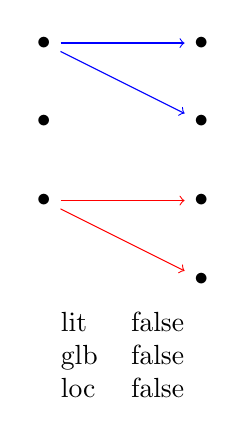
\begin{tikzpicture}[node distance = 1cm]
        % Nodes

        \node (X-1) {$\Large{\bullet}$};

        \node (X-2) [below of = X-1] {$\Large{\bullet}$};

        \node (X-3) [below of = X-2] {$\Large{\bullet}$};

        \node (Y-1) [right of = X-1, node distance = 2cm]{$\Large{\bullet}$};

        \node (Y-2) [below of = Y-1] {$\Large{\bullet}$};

        \node (Y-3) [below of = Y-2] {$\Large{\bullet}$};

        \node (Y-4) [below of = Y-3] {$\Large{\bullet}$};

        % table added from here

        \node (X-4) [below of = X-3, node distance = 2cm] {};

        \node (table) [right of = X-4] {
          \begin{tabular}{ll}
            \lit & false \\
            \glb & false \\
            \loc & false 
          \end{tabular}};

        % Arrows

        \path [draw=blue,->] (X-1) -> (Y-1);

        \path [draw=blue,->] (X-1) -> (Y-2);


        \path [draw=red,->] (X-3) -> (Y-3);

        \path [draw=red,->] (X-3) -> (Y-4);

      \end{tikzpicture}

}
\subfloat[fig:literal][literal]{
  \label{fig:literal-AE}

  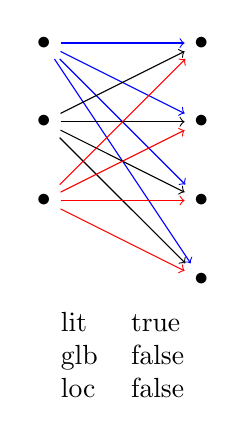
\begin{tikzpicture}[node distance = 1cm]
        % Nodes

        \node (X-1) {$\Large{\bullet}$};

        \node (X-2) [below of = X-1] {$\Large{\bullet}$};

        \node (X-3) [below of = X-2] {$\Large{\bullet}$};

        \node (Y-1) [right of = X-1, node distance = 2cm]{$\Large{\bullet}$};

        \node (Y-2) [below of = Y-1] {$\Large{\bullet}$};

        \node (Y-3) [below of = Y-2] {$\Large{\bullet}$};

        \node (Y-4) [below of = Y-3] {$\Large{\bullet}$};

        % table added from here

        \node (X-4) [below of = X-3, node distance = 2cm] {};

        \node (table) [right of = X-4] {
          \begin{tabular}{ll}
            \lit & true \\
            \glb & false \\
            \loc & false 
          \end{tabular}};

        % Arrows

        \path [draw=blue,->] (X-1) -> (Y-1);

        \path [draw=blue,->] (X-1) -> (Y-2);

        \path [draw=blue,->] (X-1) -> (Y-3);

        \path [draw=blue,->] (X-1) -> (Y-4);


        \path [draw=black,->] (X-2) -> (Y-1);

        \path [draw=black,->] (X-2) -> (Y-2);

        \path [draw=black,->] (X-2) -> (Y-3);

        \path [draw=black,->] (X-2) -> (Y-4);



        \path [draw=red,->] (X-3) -> (Y-1);

        \path [draw=red,->] (X-3) -> (Y-2);

        \path [draw=red,->] (X-3) -> (Y-3);

        \path [draw=red,->] (X-3) -> (Y-4);

      \end{tikzpicture}

}
\subfloat[fig:weak][weak]{
  \label{fig:weak}

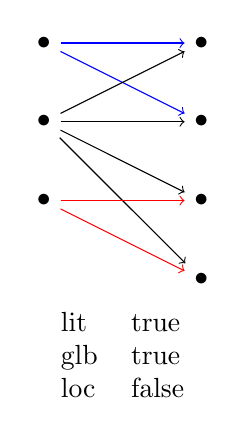
\begin{tikzpicture}[node distance = 1cm]
        % Nodes

        \node (X-1) {$\Large{\bullet}$};

        \node (X-2) [below of = X-1] {$\Large{\bullet}$};

        \node (X-3) [below of = X-2] {$\Large{\bullet}$};

        \node (Y-1) [right of = X-1, node distance = 2cm]{$\Large{\bullet}$};

        \node (Y-2) [below of = Y-1] {$\Large{\bullet}$};

        \node (Y-3) [below of = Y-2] {$\Large{\bullet}$};

        \node (Y-4) [below of = Y-3] {$\Large{\bullet}$};

        % table added from here

        \node (X-4) [below of = X-3, node distance = 2cm] {};

        \node (table) [right of = X-4] {
          \begin{tabular}{ll}
            \lit & true \\
            \glb & true \\
            \loc & false 
          \end{tabular}};

        % Arrows

        \path [draw=blue,->] (X-1) -> (Y-1);

        \path [draw=blue,->] (X-1) -> (Y-2);


        \path [draw=black,->] (X-2) -> (Y-1);

        \path [draw=black,->] (X-2) -> (Y-2);

        \path [draw=black,->] (X-2) -> (Y-3);

        \path [draw=black,->] (X-2) -> (Y-4);


        \path [draw=red,->] (X-3) -> (Y-3);

        \path [draw=red,->] (X-3) -> (Y-4);

      \end{tikzpicture}


}
\subfloat[fig:strong][strong]{
  \label{fig:strong}

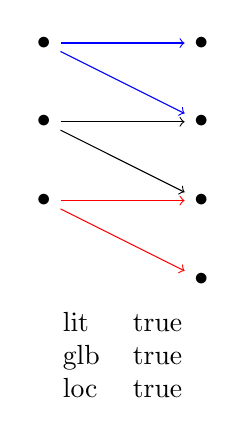
\begin{tikzpicture}[node distance = 1cm]
        % Nodes

        \node (X-1) {$\Large{\bullet}$};

        \node (X-2) [below of = X-1] {$\Large{\bullet}$};

        \node (X-3) [below of = X-2] {$\Large{\bullet}$};

        \node (Y-1) [right of = X-1, node distance = 2cm]{$\Large{\bullet}$};

        \node (Y-2) [below of = Y-1] {$\Large{\bullet}$};

        \node (Y-3) [below of = Y-2] {$\Large{\bullet}$};

        \node (Y-4) [below of = Y-3] {$\Large{\bullet}$};

        % table added from here

        \node (X-4) [below of = X-3, node distance = 2cm] {};

        \node (table) [right of = X-4] {
          \begin{tabular}{ll}
            \lit & true \\
            \glb & true \\
            \loc & true 
          \end{tabular}};

        % Arrows

        \path [draw=blue,->] (X-1) -> (Y-1);

        \path [draw=blue,->] (X-1) -> (Y-2);


        \path [draw=black,->] (X-2) -> (Y-2);

        \path [draw=black,->] (X-2) -> (Y-3);


        \path [draw=red,->] (X-3) -> (Y-3);

        \path [draw=red,->] (X-3) -> (Y-4);

      \end{tikzpicture}



}

  \caption{Distinguishing scenarious for \as-sentences}
  \label{fig:AS-distinguishing-pics}
\end{figure}


\subsection{\es-sentences}
\label{sec:es-sentences}

The situation for \es-sentences like (\ref{bsp:GE}) is similar, but a
little more complicated because the embedding quantifier is
non-monotonic. Again, we consider a literal reading as in
(\ref{bsp:GE-Literal}), a global reading as in (\ref{bsp:GE-Global})
and a local reading as in (\ref{bsp:GE-Local}).

\begin{exer}{bsp:GE}
\ex \mymark{Exactly one} of the students read {\mymark{some}} of the
  papers.

  \begin{xlist}
  \ex \mymark{Exactly one} of the students read
    {\mymark{some and maybe all}} of the papers. \hfill (\es-\lit)
  \ex 
    \mymark{Exactly one} of the students read \mymark{some and maybe all} 
    and  \hfill (\es-\glb)\\
    it's not the case that \mymark{exactly one} of the students read \mymark{all} of the papers.
  \ex 
    \mymark{Exactly one} of the students read {\mymark{some  but not all}} of the
    papers. \hfill (\es-\loc)
  \end{xlist}
\end{exer}

\noindent Entailment relations in this case are non-linear:
\begin{exe}
  \ex \label{bsp:Entailments-GE}       \lit\ $\supset$ \glb\ $\color{mycol}{\subset}$ \loc 
    % \hspace{1cm} and \hspace{1cm}  \lit\ $\not \supset$ \loc
\end{exe}
Of course, $\glb \subseteq \lit$ by definition of global readings. But
the entailment is asymmetric, because the extra information that it is
not the case that exactly one student read all of the papers is not
entailed by the literal reading (\ref{bsp:GE-Literal}). However,
unlike for \as-sentences, \loc is not stronger than \glb, but
asymmetrically entailed by the latter. To see this, notice that the
global reading is equivalent to:

\begin{exe}
  \exp{bsp:GE-Global} \mymark{Exactly one} of the students read \mymark{some but not
    all} and \\
  \mymark{everybody else} read \mymark{none} of the papers.
\end{exe}

\noindent This reformulation also makes clear that \loc and \lit are
logically independent.

Given these entailment relations, there are again four different
situations, named following \citet{ChemlaSpector2010:Experimental-Ev},
corresponding to the four possible distributions of truth values:

\begin{center}
  \begin{tabular}{lccc}
    \toprule
    situation    & \multicolumn{3}{c}{truth value} 
  \\ 
  \cmidrule(r){2-4}
    & \textsc{lit} & \textsc{glb} & \textsc{loc} \\ \midrule
    false   & 0 & 0 & 0 \\
    literal & 1 & 0 & 0 \\
    local   & 0 & 0 & 1 \\
    all     & 1 & 1 & 1 \\ \bottomrule
  \end{tabular}
\end{center}

\noindent Examples for each situation are given in
Figure~\ref{fig:ES-distinguishing-pics}. Again there several possible
scenarios within each truth-value distribution, except for the literal
situation in \ref{fig:literal-GE}.



\begin{figure}[]
  \centering
  
\subfloat[fig:false][false]{
  \label{fig:false-GE}

  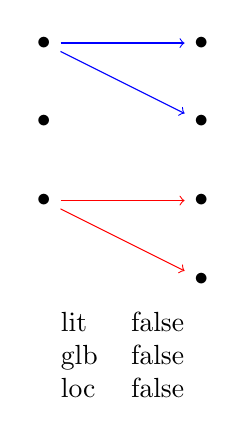
\begin{tikzpicture}[node distance = 1cm]
        % Nodes

        \node (X-1) {$\Large{\bullet}$};

        \node (X-2) [below of = X-1] {$\Large{\bullet}$};

        \node (X-3) [below of = X-2] {$\Large{\bullet}$};

        \node (Y-1) [right of = X-1, node distance = 2cm]{$\Large{\bullet}$};

        \node (Y-2) [below of = Y-1] {$\Large{\bullet}$};

        \node (Y-3) [below of = Y-2] {$\Large{\bullet}$};

        \node (Y-4) [below of = Y-3] {$\Large{\bullet}$};

        % table added from here

        \node (X-4) [below of = X-3, node distance = 2cm] {};

        \node (table) [right of = X-4] {
          \begin{tabular}{ll}
            \lit & false \\
            \glb & false \\
            \loc & false 
          \end{tabular}};


        % Arrows

        \path [draw=blue,->] (X-1) -> (Y-1);

        \path [draw=blue,->] (X-1) -> (Y-2);


        \path [draw=red,->] (X-3) -> (Y-3);

        \path [draw=red,->] (X-3) -> (Y-4);

      \end{tikzpicture}


}
\subfloat[fig:literal][literal]{
  \label{fig:literal-GE}

      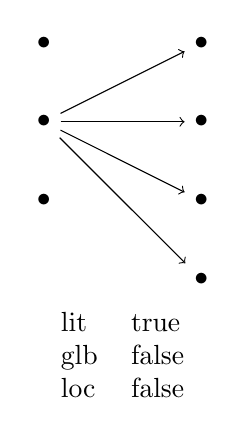
\begin{tikzpicture}[node distance = 1cm]
        % Nodes

        \node (X-1) {$\Large{\bullet}$};

        \node (X-2) [below of = X-1] {$\Large{\bullet}$};

        \node (X-3) [below of = X-2] {$\Large{\bullet}$};

        \node (Y-1) [right of = X-1, node distance = 2cm]{$\Large{\bullet}$};

        \node (Y-2) [below of = Y-1] {$\Large{\bullet}$};

        \node (Y-3) [below of = Y-2] {$\Large{\bullet}$};

        \node (Y-4) [below of = Y-3] {$\Large{\bullet}$};

        % table added from here

        \node (X-4) [below of = X-3, node distance = 2cm] {};

        \node (table) [right of = X-4] {
          \begin{tabular}{ll}
            \lit & true \\
            \glb & false \\
            \loc & false 
          \end{tabular}};

        % Arrows

        \path [draw=black,->] (X-2) -> (Y-1);

        \path [draw=black,->] (X-2) -> (Y-2);

        \path [draw=black,->] (X-2) -> (Y-3);

        \path [draw=black,->] (X-2) -> (Y-4);

      \end{tikzpicture}

}
\subfloat[fig:local][local]{
  \label{fig:local}

            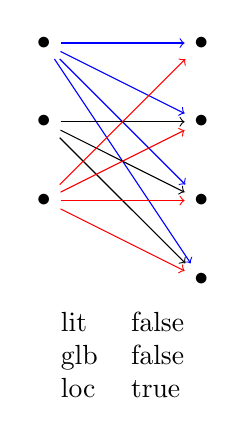
\begin{tikzpicture}[node distance = 1cm]
        % Nodes

        \node (X-1) {$\Large{\bullet}$};

        \node (X-2) [below of = X-1] {$\Large{\bullet}$};

        \node (X-3) [below of = X-2] {$\Large{\bullet}$};

        \node (Y-1) [right of = X-1, node distance = 2cm]{$\Large{\bullet}$};

        \node (Y-2) [below of = Y-1] {$\Large{\bullet}$};

        \node (Y-3) [below of = Y-2] {$\Large{\bullet}$};

        \node (Y-4) [below of = Y-3] {$\Large{\bullet}$};

        % table added from here

        \node (X-4) [below of = X-3, node distance = 2cm] {};

        \node (table) [right of = X-4] {
          \begin{tabular}{ll}
            \lit & false \\
            \glb & false \\
            \loc & true 
          \end{tabular}};

        % Arrows

        \path [draw=blue,->] (X-1) -> (Y-1);

        \path [draw=blue,->] (X-1) -> (Y-2);

        \path [draw=blue,->] (X-1) -> (Y-3);

        \path [draw=blue,->] (X-1) -> (Y-4);



        \path [draw=black,->] (X-2) -> (Y-2);

        \path [draw=black,->] (X-2) -> (Y-3);

        \path [draw=black,->] (X-2) -> (Y-4);



        \path [draw=red,->] (X-3) -> (Y-1);

        \path [draw=red,->] (X-3) -> (Y-2);

        \path [draw=red,->] (X-3) -> (Y-3);

        \path [draw=red,->] (X-3) -> (Y-4);

      \end{tikzpicture}

}
\subfloat[fig:all][all]{
  \label{fig:all}

      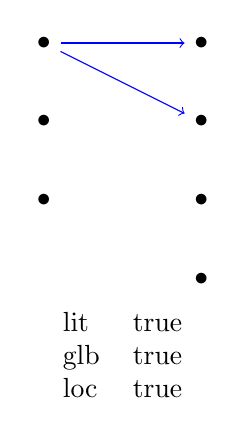
\begin{tikzpicture}[node distance = 1cm]
        % Nodes

        \node (X-1) {$\Large{\bullet}$};

        \node (X-2) [below of = X-1] {$\Large{\bullet}$};

        \node (X-3) [below of = X-2] {$\Large{\bullet}$};

        \node (Y-1) [right of = X-1, node distance = 2cm]{$\Large{\bullet}$};

        \node (Y-2) [below of = Y-1] {$\Large{\bullet}$};

        \node (Y-3) [below of = Y-2] {$\Large{\bullet}$};

        \node (Y-4) [below of = Y-3] {$\Large{\bullet}$};

        % table added from here

        \node (X-4) [below of = X-3, node distance = 2cm] {};

        \node (table) [right of = X-4] {
          \begin{tabular}{ll}
            \lit & true \\
            \glb & true \\
            \loc & true 
          \end{tabular}};

        % Arrows

        \path [draw=blue,->] (X-1) -> (Y-1);

        \path [draw=blue,->] (X-1) -> (Y-2);

      \end{tikzpicture}

}

  \caption{Distinguishing scenarious for \es-sentences}
  \label{fig:ES-distinguishing-pics}

\end{figure}


\section{Theories and predictions}
\label{sec:theories-predictions}

With some mild simplification, we can distinguish three main
theoretical positions that make different predictions about the
available and preferred readings of \as- and \es-sentences
\citep[c.f.][for
overview]{Horn2006:The-Border-Wars,Geurts2010:Quantity-Implic,Sauerland2012:The-Computation}. We
will refer to these here as \mymark{traditionalism},
\mymark{conventionalism} and \mymark{grammaticalism} and treat each
one in turn. Since there is some leeway in assessing the predictions
for some of these positions (depending on which of several reasonable
additional assumptions we should adopt), we will distinguish different
varieties of each position. For convenience, the predictions of each
(variety of each) position are also summarized in
Table~\ref{tab:predictions} at the end of this section.

\subsection{Traditionalism}
\label{sec:traditionalism}

We refer to traditionalism as traditionalism because of its
conservative stance towards Grice's original theory of conversational
implicatures \citep{Grice1975:Logic-and-Conve}. Many author's have
defended traditionalist positions in this sense. Of the more recent
literature, we would consider as traditionalist, among others,
contributions such as by
\citet{Spector2006:Scalar-Implicat,Sauerland2004:Scalar-Implicat,Russell2006:Against-Grammat,vanRooijSchulz:ExhaustiveInterpretation,Geurts2010:Quantity-Implic,Franke2011:Quantity-Implic}. 

 According to Grice,
conversational implicatures, of which quantity/scalar implicatures are
a special case, are to be thought of as rationalizations of speaker
behavior. Central in this reasoning is the assumption that the
speaker's behavior is efficient (if not optimal) and
goal-oriented. Usually, the assumed goal of conversation is
cooperative exchange of helpful information from the speaker to the
hearer.

Consequently, the \mymark{Gricean recipe}
\citep[c.f.][]{Geurts2010:Quantity-Implic} for deriving a simple scalar
inference like that in (\ref{bsp:Plain-SI-Implicature}) from an
utterance of (\ref{bsp:Plain-SI-Target}) is as follows: if the issue
whether Hans solved only some or all of the problem is relevant, then
a cooperative and knowledgable speaker would utter
(\ref{bsp:Plain-SI-Alternative}) if in a position to do so; hence, one
of the most natural explanations of why such a speaker has not uttered
(\ref{bsp:Plain-SI-Alternative}), but only (\ref{bsp:Plain-SI-Target})
is that she is uncertain of whether (\ref{bsp:Plain-SI-Alternative})
is true; but on the assumption that she is knowledgeable (competent,
opinionated, informed \dots) it follows that
(\ref{bsp:Plain-SI-Implicature}) should in fact be true.\fn{We are
  glossing here somewhat swiftly over the more nuanced details of the
  derivation of implicatures targeting the speaker's epistemic state
  \citep[e.g.][]{Gazdar1979:Pragmatics:-Imp,Soames1982:How-Presupposit},
  as this is not crucially relevant for the issues we are interested
  in here.}\textsuperscript{,}\dn{do we need to enlarge on epistemic
  implicatures?}

\begin{exer}{bsp:Plain-SI}
  \ex 
    \begin{xlist}
      \ex \label{bsp:Plain-SI-Target} Hans solved \mymark{some} of the problems.
      \ex \label{bsp:Plain-SI-Implicature} $\implicates$ Hans solved
        \mymark{some but not all} of the problems.
      \ex  \label{bsp:Plain-SI-Alternative}  Hans solved \mymark{all} of the problems.
    \end{xlist}
\end{exer}

A similar line of reasoning applies immediately also to \as- and
\es-sentences and derives the global reading in a straightforward
way. Consequently, traditionalism predicts that both literal and
global readings are available: literal readings, because these form
the starting point of pragmatic reasoning; global readings because
these may be arrived at by the Gricean recipe.

Whether traditionalism predicts a preference for global or literal
readings depends on whether the auxiliary assumptions necessary to
derive global readings by the Gricean recipe are plausibly met in the
particular case of utterance of \as- and \es-sentences. These
auxiliary assumptions include relevance of the extra information
provided in the global reading, mutual awareness that the stronger
alternative has been a speaker option, the speaker's competence about
the issue, etc. Normally, traditionalist accounts would assume that
these extra assumptions are met. In that case, traditionalism would
predict that the global readings should be preferred over the literal
readings. On the other hand, it might also be hypothesized that, for
example, a competence assumption is harder to justify for \as- and
\es-sentences in general than for simpler sentences such as
(\ref{bsp:Plain-SI}), because of the additional quantificational
element: it might be less clear that the speaker knows exactly how
many students solved how many problems, than that the speaker knows
exactly how many problems, e.g., Hans solved. In that case, or if any
other assumption of the Gricean recipe cannot be maintained,
traditionalism would predict that the literal reading would be
preferred over the global one. But that means that there are at least
two varieties of traditionalism that, depending on which additional
assumptions we would make, yield slightly different predictions:
\mymark{the strong variety of traditionalism} maintains that the
auxiliary assumptions of the Gricean recipe hold
usually/strongly/unless-completely-intenable and therefore predicts
that global readings are preferred over the literal ones; \mymark{the
  weak variety of traditionalism} holds that the auxiliary assumptions
are more fragile and predicts that literal readings are preferred over
the global ones.\fn{For clarity: although weak traditionalism does not
  predict the global reading to be preferred, it would might or might
  no still predict an epistemically weak implicature, similar to the
  global reading, that the speaker is uncertain whether the stronger
  alternative is true. Whether it does predict that depends on which
  auxiliary assumption are assumed to be met and which are
  not.}\dn{acknowledge comment by Philippe Schlenker here}

What about the local reading then? Here, the situation is slightly
different for \as- and the \es-sentences. Look at \es-sentences
first. Traditionalism does not predict that a local reading is
available for \es-sentences, at least not as a quantity implicature
\citep[c.f.][]{GeurtsPouscoulous2009:Embedded-Implic,ChemlaSpector2010:Experimental-Ev}. This
is because traditionalism assumes that quantity implicatures are
pragmatic enrichments of the literal meaning of an utterance, obtained
by conjoining the literal meaning with a suitable set of negated
alternatives. But since the literal and the local reading of
\es-sentences are logically independent, there is no way that local
readings can be derived in a traditionalist manner as a quantity
implicature. Traditionalism often does concede that (something like)
local readings can occur if scalar items are marked with \emph{special
  intonation}, albeit then as a signal of a different pragmatic
process
\citep[e.g.][]{Horn2006:The-Border-Wars,Geurts2009:Scalar-Implicat,Geurts2010:Quantity-Implic}. We
will come back to this issue in Section~\ref{sec:role-intonation}.

On the other hand, as for \as-sentences, there is a traditionalist way
of deriving the local implicature, namely by assuming that not only
(\ref{bsp:AE-Alternative}) is an alternative to (\ref{bsp:AE}), but
also the sentence in (\ref{bsp:AE-Alternatives-Extended}).

\begin{exer}{bsp:AE}
  \ex \mymark{All} of the students solved \mymark{some} of the problems.
\end{exer}

\begin{exer}{bsp:AE-Alternative}
  \ex \mymark{All} of the students solved \mymark{all} of the problems.
\end{exer}

\begin{exe}
\ex \label{bsp:AE-Alternatives-Extended} \mymark{Some} of the students solved \mymark{all} of the problems.
\end{exe}

\noindent Clearly, if we conjoin a literal reading of (\ref{bsp:AE})
with the negation of (\ref{bsp:AE-Alternatives-Extended}) we obtain
exactly the local reading. (Notice that the negation of
(\ref{bsp:AE-Alternatives-Extended}) entails the negation of
(\ref{bsp:AE-Alternative}), so it makes no difference (not) to add it
in this case.) Consequently, traditionalism does predict that the
local reading of \as-sentences is available if
(\ref{bsp:AE-Alternatives-Extended}) is an available alternative. We
should therefore introduce another distinction: \mymark{restricted
  traditionalism} assumes that (\ref{bsp:AE-Alternatives-Extended}) is
not available and therefore predicts that the local reading for
\as-sentences is not available; in contrast, \mymark{unrestricted
  traditionalism} assumes that (\ref{bsp:AE-Alternatives-Extended}) is
available and so is the local reading.

Still, even unrestricted traditionalism would not predict that the
local reading is preferred over the global reading. This is because
the derivation of the local implicature via
(\ref{bsp:AE-Alternatives-Extended}) hinges on yet another auxiliary
assumption, namely the availability of the alternative in
(\ref{bsp:AE-Alternatives-Extended}), which seems much less obvious
and therefore presumably is less readily available than the
alternative in (\ref{bsp:AE-Alternative}). Consequently, we derive the
following predictions about preferences for unrestricted
traditionalism: weak unrestricted traditionalism prefers the literal
over the global over the local reading, while strong unrestricted
traditionalism prefers the global over the local over the literal
reading. The predictions for all of the relevant theoretical positions
are also summarized in Table~\ref{tab:predictions}.


\subsection{Conventionalism}
\label{sec:conventionalism}

Lexical conventionalism is a position that has been defended only by a
minority
\citep{LevinsonPresumptiveMeanings2000,Chierchia:2004_ScalarImplicatures}. This
notwithstanding, the position is \emph{prima facie} highly plausible
as well.\fn{Compare also \citet{Sauerland2012:The-Computation} who
  argues quite favorably for a pragmatically informed conventionalism,
  although eventually dismissing it in favor of grammaticalism.} The
general idea is that the upper-bounding inference from \emph{some} to
\emph{some but not all} occurs so frequently that it would be
inefficient to go over and over again through the kind of Gricean
reasoning that traditionalists propose. Conventionalism therefore
assumes that the scalar inferences has become routinized, hard-wired,
so much so that there are two lexical entries for a scalar item like
\emph{some}, one with meaning \emph{some and maybe all} and one with
the meaning \emph{some but not all}.

\citet{LevinsonPresumptiveMeanings2000} proposed that the latter is
the preferred default meaning. Call this position
\mymark{defaultism}. Levinson's defaultism has strong empirical
evidence against it, because several processing studies show that the
computation of scalar inferences appears to be time- and
effort-consuming, when they \emph{do} arise, not when they
\emph{don't}, as defaultism would have it
\citep[c.f.][]{BrehenyKatsos2006:Are-Generalised,BrehenyKatsos2008:Experimental-In,NeysDe-NeysSchaeken2007:When-People-Are}.\fn{But
  there is also competing evidence that scalar inferences are
  immediate, low-level processes
  \citep{GrodnerKlein2010:Some-and-Possib}.}\dn{more references!} For
completeness sake, let's call \mymark{literalism}\dn{better name?} the
opposite view that the literal meanings are \emph{ceteris paribus}
preferred. We are not aware that anyone has defended this option, but
we will come back to this later on.

Both varieties of conventionalism make interesting predictions about
available readings for \as- and \es-sentences. Unaided,
conventionalism does not predict that global readings are
available. The lexically stored upper-bound for scalar \emph{some}
only allows to derive literal and local readings. Moreover, defaultism
predicts that local readings are preferred over literal ones. Contrary
to that, our dummy position of literalism predicts that literal
readings are preferred over local ones.

\subsection{Grammaticalism}
\label{sec:grammaticalism}

The third and final kind of theoretical position we should consider
here is \mymark{grammaticalism}. It is safe to say that grammaticalism
is currently \emph{en vogue} with ever more very sophisticated
theoretical evidence (i.e., evidence based on intuitive judgements and
more theoretical considerations) being excavated in its favor
\citep[c.f.][]{Chierchia2006:Broaden-Your-Vi,Fox2007:Free-Choice-and,Magri2011:Another-Argumen,Sauerland2012:The-Computation,ChierchiaFox2008:The-Grammatical,Chierchia2012:FC-Nominals-and}. When
it comes to the predictions of available readings of \as- and
\es-sentences, grammaticalism looks a bit like the conjunction of
traditionalism and conventionalism. But conceptually speaking,
grammaticalism goes down a road of its own.

Grammaticalism approaches quantity implicatures by postulating a
silent operator that can be variably applied during compositional
computation of a sentence's truth-value
\citep{Chierchia2006:Broaden-Your-Vi}, if necessary multiple times
\citep{Fox2007:Free-Choice-and}. This silent operator is variably
referred to as $\mathrm{O}(\cdot)$ or $\exh(\cdot)$, because it is
assumed to be similar in effect to the meaning of particle \emph{only}
or of the mechanism of \emph{exhaustive interpretation}
\citep{GroenendijkStokhofThesis1984,Stechowvon-StechowZimmermann1984:Term-Answers-an,Rooijvan-RooijSchulz2013:Exhaustive-Inte,vanRooijSchulz:ExhaustiveInterpretation,Fox2007:Free-Choice-and}. For
our purposes here, it is enough to note that $\exh(\cdot)$ is a
poly-typed function that enriches an expression $X$, which crucially
need not be a full proposition, based on a set of (suitable, relevant)
alternatives to $X$, $\alt(X)$, that yields an enriched meaning of the
form:\fn{More sophisticated formulations of exhaustive interpretation
  have been proposed
  \citep[e.g.][]{Schulz2005:A-Pragmatic-Sol,vanRooijSchulz:ExhaustiveInterpretation,Spector2006:Scalar-Implicat,Fox2007:Free-Choice-and}
  but this simple formulation is sufficient for the purposes of this
  paper. Also, we gloss here over non-trivial details in the way this
  operation is to be specified exactly within a compositional
  semantics, so as to also apply to sub-propositional expressions
  \citep{Chierchia2006:Broaden-Your-Vi}.}
\begin{exe}
  \ex \label{bsp:Exh-Def} $\exh(X,\alt(X)) = X \bigwedge_{A \in
      \alt(X)} \neg A$.
\end{exe}

As this operator can apply at various scope sites, the grammatical
approach predicts that all three readings of \as- and \es-sentences
are available: literal readings arise if no exhaustification operator
is applied; global readings arise if the exhaustification operator
takes sentence-wide scope as in (\ref{Grammar-Global}); and local
readings arise if the exhaustification operator takes scope under the
respective quantifiers as in (\ref{Grammar-Local}).

\begin{exe}
  \ex \label{Grammar-Global}
    \begin{xlist}
      \ex \label{Grammar-Global-AE} \mymark{$\exh$}(\mymark{All} of the students solved
        \mymark{some} of the problems)
      \ex \label{Grammar-Global-GE} \mymark{$\exh$}(\mymark{Exactly one} of the students solved
        \mymark{some} of the problems)
    \end{xlist}
\end{exe}

\begin{exe}
  \ex \label{Grammar-Local}
    \begin{xlist}
      \ex \label{Grammar-Local-AE} \mymark{All} of the students \mymark{$\exh$}(solved
        \mymark{some} of the problems)
      \ex \label{Grammar-Local-GE} \mymark{Exactly one} of the
        students \mymark{$\exh$}( solved
        \mymark{some} of the problems)
    \end{xlist}
\end{exe}

It is obvious that the grammatical approach, as described so far, is
rather flexible in that it makes many readings available. It is so
flexible, in fact, that it must be constrained in some way or other to
shield the approach against overgeneration. The easiest examples where
this is crucial are occurrences of scalar items in downward-entailing
environments, such as in:

\begin{exe}
\ex \label{bsp:Overgenereation-target} It's \mymark{not} the case that
  Hans solve \mymark{some} of the problems.
\end{exe}

\noindent But an assertion of normally would be taken to convey
(\ref{bsp:Overgenereation-implicature-attested}), not he disjunctive
meaning in (\ref{bsp:Overgenereation-implicature-UNattested}).

\begin{exe}
\ex 
  \begin{xlist}
  \ex \label{bsp:Overgenereation-implicature-attested} Hans solves \mymark{none} of the problems.
  \ex \label{bsp:Overgenereation-implicature-UNattested} Hans solved
    \mymark{none or all} of the problems 
  \end{xlist}
\end{exe}

\noindent The latter, however, is a reading that grammaticalism
predicts to be available, if the $\exh(\cdot)$-operator takes scope
under the negation, as in:

\begin{exe}
\ex It's not the case that Hans solved \mymark{$\exh$}(\mymark{some} of the problems)
\end{exe}

\noindent Indeed, this reading is not unattested, for witness a
continuation of (\ref{bsp:Overgenereation-target}) as in:
\begin{exe}
\ex \label{bsp:Overgeneration-continued} It's \mymark{not} the case that Hans
  solve \mymark{\emph{some}} of the problems. He solved
  \mymark{\emph{all}} of them.
\end{exe}

\noindent But this reading does seem to be marked, in that it requires
exceptional contextual circumstances and a non-standard intonational
stress. 

To account for the markedness of certain examples, grammaticalism is
therefore aided by a principle that specifies which readings are to be
preferred if several readings are generated by optional applications
of $\exh(\cdot)$ in the compositional computation of semantic
values. The principle that grammaticalists adhere to
\citep[c.f.][]{FoxSpector:Economy-and-Emb,ChierchiaFox2008:The-Grammatical,Chierchia2012:FC-Nominals-and}
is the \mymark{strongest meaning hypothesis} of
\citet{DalrympleKanazawa1998:Reciprocal-Expr}. If a given sentence has
several conceivable readings, the strongest meaning hypothesis selects
for the strongest of these. But this is only a rough
formulation. Details might
matter. \citet{ChierchiaFox2008:The-Grammatical} discuss two variants
of the strongest meaning hypothesis. Towards a formal definition, fix
a sentence with propositional content $S$ with candidate readings
$C(S)$, where $C(S)$ contains $S$ and all readings derivable from
inserting $\exh(\cdot)$ at suitable scope sites.  Then define
\emph{ceteris paribus} preferences among members of $X,Y \in C(S)$ as
a stronger partial relation:
\begin{exe}
\ex \label{bsp:SMH-Total} 
  $X > Y$ iff $X \subset Y$ 
  \attrib{\citep[(104)]{ChierchiaFox2008:The-Grammatical}}
\end{exe}
or a weaker partial relation:\dn{mention that ill-defined}
\begin{exe}
\ex \label{bsp:SMH-Partial}  $X > Y$ if $X \subset Y$ and $X$ and $Y$ are readings obtained
  from applications of $\exh(\cdot)$ at exactly the same scope sites,
  except for one 
  \attrib{\citep[(105)]{ChierchiaFox2008:The-Grammatical}}
\end{exe}
In the following we will speak of \mymark{strong grammaticalism} or
\mymark{weak grammaticalism}, depending on whether
(\ref{bsp:SMH-Total}) or (\ref{bsp:SMH-Partial}) is used.

These two varieties of grammaticalism give rise to different
predictions about preferred readings. It is easy to see that the
preference on readings that strong grammaticalism predicts is just a
mirror of the entailment relations in (\ref{bsp:Entailments-AS}) and
(\ref{bsp:Entailments-GE}): for \as-sentences strong grammaticalism
predicts that local readings are preferred over global readings which
in turn are preferred over literal readings; for \es-sentences strong
grammaticalism predicts that global readings are most preferred, while
literal and local readings are not ranked with respect to
preference. Weak grammaticalism, on the other hand, predicts that both
\as- and \es-sentences preferably get either a local or a global
reading rather than a literal reading. But weak grammaticalism does
not rank these former two with respect to each other because they
differ in more than one application of the $\exh(\cdot)$
operator. These predictions are all summarized also in
Table~\ref{tab:predictions}.

\begin{table}[t]
  \centering
  \begin{tabular}{lcccccc}
    & \multicolumn{4}{c}{availability} 
    & \multicolumn{2}{c}{preference}
    \\ \cmidrule(r){2-5}  \cmidrule(r){6-7}
    theory
    & \as-\glb
    & \as-\loc
    & \es-\glb
    & \es-\loc
    & \as
    & \es
    \\ \midrule
    traditionalism
    \\
    \ \ weak restricted 
    & $\checkmark$
    & $-$
    & $\checkmark$
    & $-$
    & \lit > \glb 
    & \lit > \glb
    \\
    \ \ weak unrestricted
    & $\checkmark$
    & $\checkmark$
    & $\checkmark$
    & $-$
    & \lit > \glb > \loc 
    & \lit > \glb
    \\
    \ \ strong restricted
    & $\checkmark$
    & $-$
    & $\checkmark$
    & $-$
    & \glb > \lit 
    & \glb > \lit
    \\
    \ \ strong unrestricted
    & $\checkmark$
    & $\checkmark$
    & $\checkmark$
    & $-$
    & \glb > \loc > \lit 
    & \glb > \lit
    \\
    conventionalism
    \\
    \ \ defaultism
    & $-$
    & $\checkmark$
    & $-$
    & $\checkmark$
    & \loc >  \lit 
    & \loc >  \lit
    \\
    \ \ literalism
    & $-$
    & $\checkmark$
    & $-$
    & $\checkmark$
    & \lit >  \loc 
    & \lit >  \loc
    \\
    grammaticalism
    \\
    \ \ total
    & $\checkmark$
    & $\checkmark$
    & $\checkmark$
    & $\checkmark$
    & \loc > \glb > \lit 
    & \glb > \lit, \loc
    \\
    \ \ partial
    & $\checkmark$
    & $\checkmark$
    & $\checkmark$
    & $\checkmark$
    & \glb, \loc > \lit 
    & \glb, \loc >  \lit
    \\
  \end{tabular}
  \caption{Predictions of the relevant theoretical positions}
  \label{tab:predictions}
\end{table}




\section{Previous studies}
\label{sec:previous-studies}

The rather divergent predictions made by rivaling theoretical
positions call for empirical testing. Indeed, a small number of
studies have gathered useful evidence. The following briefly reviews
the studies of \citet{GeurtsPouscoulous2009:Embedded-Implic},
\citet{CliftonDube2010:Embedded-Implic} and
\citet{ChemlaSpector2010:Experimental-Ev}. Unfortunately, the
conjoined evidence from all of these studies is inconclusive as to the
availability of local readings. Moreover, we argue that the question
of which reading is preferred for \as- and \es-sentences is only
insufficiently addressed by previous studies.

\subsection{\citet{GeurtsPouscoulous2009:Embedded-Implic}}
\label{sec:Geurts-and-Pouscoulous}

\citet{GeurtsPouscoulous2009:Embedded-Implic} conducted a
picture-verification task to find out whether local readings of \as-
and \es-sentences are available.\fn{Actually,
  \citet{GeurtsPouscoulous2009:Embedded-Implic} did not use
  \es-sentences, but sentences where scalar \emph{some} was embedded
  under non-monotonic quantifier \emph{exactly two} (with appropriate
  pictures, of course). This case is a little more complex, but we
  will gloss over this here, treating their data, as it if was obtain
  for \es-sentences.} The critical conditions of their study presented
subjects with pictures like those in Figure~\ref{fig:weak} and
\ref{fig:local} where the local reading gets a different truth-value
from the literal and the global reading. In particular, for
\as-sentences the local reading is false for the critical picture in
Figure~\ref{fig:weak} whereas the literal and global readings are
true; for \es-sentences the local reading is true for the critical
picture in Figure~\ref{fig:local}, whereas the literal and global
readings are false.

The results of \citeauthor{GeurtsPouscoulous2009:Embedded-Implic} were
strikingly unambiguous: there were \emph{no} responses indicative of a
local read \emph{at all}! In other words, all of the subjects judged
\as-sentences true in a situation like in Figure~\ref{fig:weak} and
all of the subjects judged \es-sentences false in situations like
\ref{fig:local}.


\subsection{\citet{CliftonDube2010:Embedded-Implic}}
\label{sec:clifton-dube}

\citeauthor{GeurtsPouscoulous2009:Embedded-Implic} was quickly
succeeded by three commentaries: \citet{Ippolito2010:Embedded-Implic}
supported \citeauthor{GeurtsPouscoulous2009:Embedded-Implic}'s
finding, \citet{Sauerland2010:Embedded-Implic} criticized, both based
on theoretical considerations; \citet{CliftonDube2010:Embedded-Implic}
replied with a small experimental study of their
own. \citeauthor{CliftonDube2010:Embedded-Implic} really only paid
attention to \as-sentences, which is quite unfortunate. They were
worried that \citeauthor{GeurtsPouscoulous2009:Embedded-Implic}'s
picture-verification paradigm might unjustly de-emphasize local
readings for \as-sentences, because asking whether a sentence fits a
picture, as \citeauthor{GeurtsPouscoulous2009:Embedded-Implic} did,
might create a bias for accepting sentences also on a weaker,
dispreferred reading. Unfortunately, this criticism does not apply to
the non-monotonic \es-condition, where subjects unanimously
\emph{rejected} the \es-sentences, despite the fact that there was a
weaker reading, namely the local one, which could have licensed a
positive judgement.

Nonetheless, \citeauthor{CliftonDube2010:Embedded-Implic}'s
experimental data is worthwhile considering because their study was
aimed at finding out whether the local reading was preferred over the
literal reading or vice
versa. \citeauthor{CliftonDube2010:Embedded-Implic} conducted a
picture-choice task where, in the critical conditions, subjects were
presented with an \as-sentence and a pair of pictures. Subjects were
asked to ``indicate which shape is best described by the
[\as-]sentence'' and could choose either picture, or options ``both''
and ``neither.'' There were two versions of this experiment, differing
in which kind of picture pairs were presented on critical trials.

In version 1, the picture pair consisted of the weak and strong
situations in Figures~\ref{fig:weak} and
\ref{fig:strong}. The response percentages observed by
\citeauthor{CliftonDube2010:Embedded-Implic} were:

\begin{center}
  \begin{tabular}{cccc}
    weak & strong & both & neither
    \\ \midrule 
 3 & 39 & 57 & 1 
  \end{tabular}
\end{center}

\noindent That the majority answer is ``both'' could be taken as
evidence that the literal reading is the preferred one. But the almost
40\% of choices for the strong situation, so
\citeauthor{CliftonDube2010:Embedded-Implic} argue, might be
indicative of the availability of the local reading.

In version 2 of \citeauthor{CliftonDube2010:Embedded-Implic}'s
experiment, the picture pair consisted of the literal and weak
situations in Figures~\ref{fig:literal-AE} and \ref{fig:weak}. In this
case, response percentages were:

\begin{center}
  \begin{tabular}{cccc}
    weak & literal & both & neither
    \\ \midrule 
    28 & 6 & 50 & 17 
  \end{tabular}
\end{center}

\noindent Again the majority response ``both'' might speak for a
preference for the literal reading, but, as
\citeauthor{CliftonDube2010:Embedded-Implic} argue the 17\% of
``neither'' answers in this case suggest that the local reading is
available.  

Taken together, \citeauthor{CliftonDube2010:Embedded-Implic} take
these results to contradict
\citeauthor{GeurtsPouscoulous2009:Embedded-Implic}'s findings. Local
readings are, after all, attested if subjects are given a choice as to
which situation they consider most fitting for an \as-sentence.

There several problems and shortcomings with this study. First of all,
\es-sentences were not considered. Secondly, the availability and
preference of global readings was not tested for. 

problem with this study is that
data about subjects' choices about effect of a preference for one type
of situation from Figure~\ref{fig:AS-distinguishing-pics} as over
another has nothing to say about which ``shape is best described by
the [\as-]sentence''

\subsection{\citet{ChemlaSpector2010:Experimental-Ev}}
\label{sec:Chemla-Spector}


\subsection{What's missing}
\label{sec:whats-missing}

\begin{itemize}
\item independence of pictorial complexity and preference of reading
\item provide a benchmark from which to deduce preference relations
\item control for intonational pattern (present auditorily)
\end{itemize}


\subsection{The role of intonation}
\label{sec:role-intonation}

HERE OR LATER?!

\begin{itemize}
\item proposed by
  \citet{Horn2006:The-Border-Wars,Geurts2009:Scalar-Implicat,Geurts2010:Quantity-Implic},
  \citep[c.f.][]{ChemlaSpector2010:Experimental-Ev}
\end{itemize}

\newpage



\section{Design}
\label{sec:design}

\lipsum[1]

\section{Results}
\label{sec:results}

\lipsum[1]

\section{Discussion}
\label{sec:discussion}

\lipsum[1]





\printbibliography[heading=bibintoc]

\end{document}
